\section{LLM Fine-Tuning for NPU Kernels}\label{fine_tune}
% 描述ft的目的和分两步走实现的策略
% 章节5中介绍了数据集，下面我们利用SFT和RL来注入领域知识。在SFT中, 除了使用到上一章节我们构建的数据集外，我们还使用了数据飞轮的操作。具体来说我们大量的报错信息进行了数据纠正xxx。与此同时，我们还使用了强化学习来增加AscendC 的领域知识，其中我们利用SFT生成大量的算子实例，并根据算子的执行结果（编译，精度通过情况）进行评估，自动构建用于训练的正负样本对。

%我们通过两个步骤来增强LLM生成AscendC算子的能力。分别是基于基于Ascend知识增强的SFT和强化学习。在SFT知识注入后，我们还设计了一套针对算子精度问题的高质量SFT训练数据，通过处理那些SFT之后“编译通过但运行结果错误”的高难度样本，结合GT标准答案，引导大模型进行深度归因分析和从零重构。在强化学习中，我们通过对SFT之后的测试算子样例的执行结果（编译，精度通过情况）进行评估，自动构建用于训练的正负样本对。
%We enhance the LLM’s ability to generate AscendC kernels through two steps: (1) Ascend-knowledge–augmented supervised fine-tuning (SFT) and (2) reinforcement learning (RL). In the first step, we perform Ascend-specific SFT using the curated dataset described in Sec.~\ref{data_construct}. We then apply a data-flywheel: we collect challenging cases that compile but fail precision tests, pair them with ground-truth references, and use them to guide the LLM in causal analysis and reconstruction. In the second step, building on the improved SFT model, we generate a large number of kernel instances and automatically construct positive–negative training pairs based on compilation and precision results, enabling RL to further refine the model in a robust and correctness-oriented manner.

To enable reliable NPU kernel generation under strict programming constraints, we introduce \href{https://huggingface.co/AscendKernelGen/models}{\textcolor{blue}{KernelGen-LM}}, a publicly available domain-adapted model designed to internalize AscendC-specific API semantics and complex execution dependencies. Our approach employs a two-stage optimization strategy combining Supervised Fine-Tuning (SFT) and Reinforcement Learning (RL). The first stage performs NPU-aware supervised fine-tuning (SFT) with curated and iteratively refined data, enabling the model to acquire foundational knowledge of AscendC syntax, APIs, and kernel structure. The second stage further refines the model via reinforcement learning (RL) using execution-based correctness signals, encouraging the generation of kernels that are not only compilable but also numerically correct.

\subsection{Supervised Fine-Tuning with Error-Derived Supervision}

%Since the original LLM lacks AscendC knowledge for NPU kernel generation, we first construct a carefully designed dataset (see Sec.~\ref{data_construct}) to provide instruction through supervised fine-tuning (SFT). However, even after knowledge injection, the model is not yet ready for reinforcement learning due to suboptimal compilation success and computational accuracy. To address this, we perform framework-level verification on generated kernels to collect error logs, revealing the model’s limitations. We then establish an interaction mechanism between the LLM and the compilation framework to systematically identify deficiencies, generate targeted error-correction training data, and incorporate it into the pretraining dataset. This iterative process forms a data flywheel that progressively improves model performance, integrating retrieval-based augmentation from the AscendC API with kernel-level error-correction optimization.
While Ascend-aware SFT provides essential syntactic and structural knowledge, we observe that models trained solely on static supervision still exhibit frequent failures in compilation stability and numerical correctness. To improve robustness prior to RL, we introduce an \emph{error-derived supervision} strategy that augments SFT with correction data generated from real execution failures, shown in Figure~\ref{fig:error_correction}. 
\begin{wrapfigure}{l}{0.48\linewidth}
    \centering
    % \vspace{-10pt}
    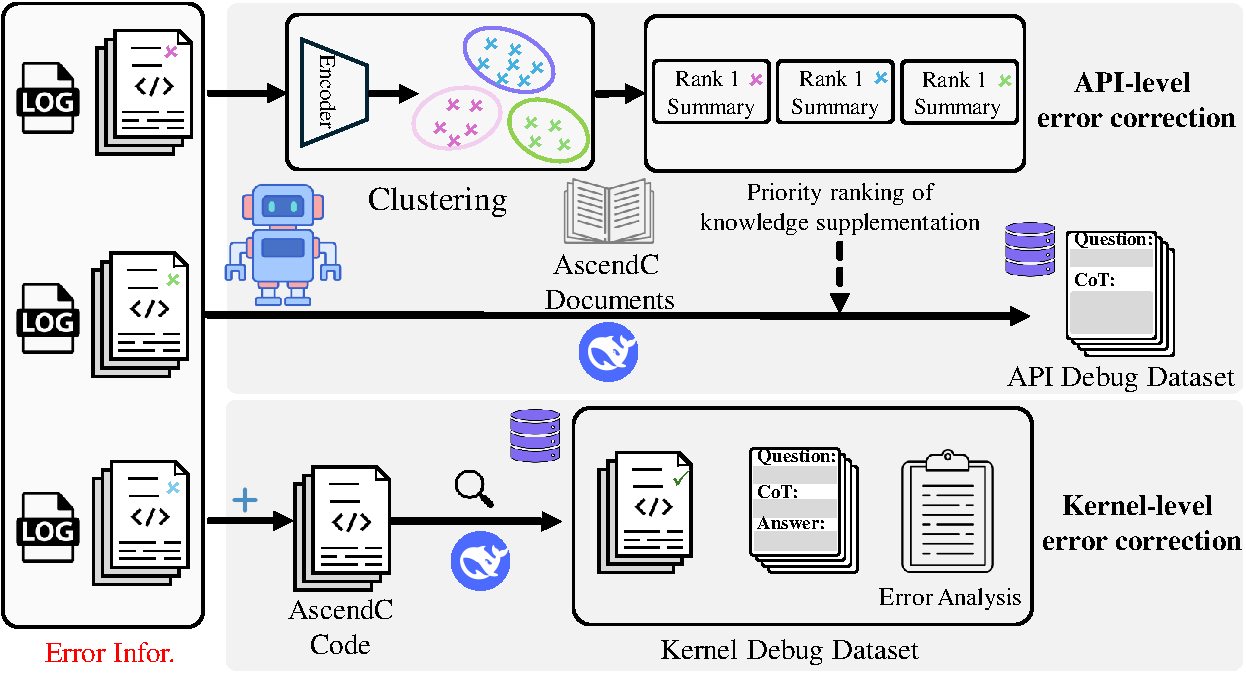
\includegraphics[width=\linewidth]{pdfs/data_debug.pdf}
    \caption{Error-Derived Supervision for API- and Kernel-Level Error Correction.}
    \vspace{-10pt}
    \label{fig:error_correction}
\end{wrapfigure}
This strategy focuses on two complementary levels of errors: API-level misuse and kernel-level numerical inconsistency.

\begin{comment}

To address this limitation, we introduce an \emph{error-derived supervision} mechanism integrated into the SFT process. Kernel generation and verification are treated as an offline data augmentation pipeline: kernels produced by the current SFT model are compiled and executed using an automatic verifier, and failure cases are systematically collected and analyzed. Execution errors, including API misuse, invalid tiling logic, and numerical inaccuracies, are transformed into structured correction examples that explicitly demonstrate the correct behavior.

This process remains fully supervised. Each newly generated sample is paired with a deterministic ground-truth target, such as corrected API invocations or reference kernel implementations, and is incorporated back into the training corpus for subsequent SFT iterations. By iteratively exposing the model to its own failure modes and providing explicit corrective supervision, the model progressively internalizes execution constraints and kernel-level invariants that are difficult to encode a priori through static data alone.

\end{comment}


%知识注入后的模型在效果上尚未达到可启动强化学习的门槛，主要表现为编译通过率与计算精度达标率仍不够理想。通过对生成算子进行框架侧验证，我们能够获取大量报错信息，这些信息清晰地揭示了模型当前的能力短板。为此，我们尝试建立模型与编译框架之间的交互机制：通过系统化识别模型缺陷，自动合成针对性的改错训练数据，并将其加入模型的预训练数据集。通过这一方式，我们正逐步构建起能够持续优化模型性能的数据飞轮


\subsubsection{API-Level Error Correction}
\label{sft_api_correction}

% Despite having constructed API invocation QA data, large language models still exhibit invocation errors, leading to high operator compilation failure rates. Therefore, we built an automated data generation pipeline to transform Ascend C operator compilation failure logs into high-quality API code debugging SFT training data. This pipeline integrates raw error logs, operator source code context, and official API documentation to automatically generate structured training samples containing "error scene + expert reasoning process + correct documentation references." The entire data construction process adopts a modular four-stage architecture, with each stage focusing on specific data transformation tasks:

% \textbf{(1) Log cleaning and extraction.} This stage filters clean error information from mixed build logs. Through regular expression matching of [ERROR] marker blocks, it automatically removes successfully compiled samples and stores error logs in a flattened structure, establishing a clean data foundation for subsequent analysis.

% \textbf{(2) Error analysis and strategic filtering.} This stage utilizes large language models for root cause analysis and error type classification, while identifying "low-pass-rate" difficult operators by calculating operator compilation pass rates. This dual filtering mechanism ensures subsequent processing focuses on the most challenging and valuable training samples.

% \textbf{(3) Contextual diagnostic report generation.} This is the core stage of the entire pipeline. The system automatically correlates three types of information sources: 1) specific error messages from error logs; 2) erroneous invocations and their context in source code (including variable definition backtracing); 3) correct usage instructions from official API documentation. These three elements are physically concatenated to form structured Markdown diagnostic reports, providing complete problem scenes for expert-level reasoning.

% \textbf{(4) SFT data synthesis.} Based on diagnostic reports, large language models act as domain experts to generate high-quality conversational data containing chain-of-thought reasoning. The system automatically performs data balancing (downsampling high-frequency errors) and data augmentation (generating diverse phrasings for low-frequency errors), and filters out invalid samples with insufficient information.

At the API level, we construct an error-correction dataset from real AscendC compilation failures. Given a compiler error log, the corresponding kernel context, and relevant official documentation, the model is trained to identify the root cause of the failure and produce a corrected implementation. This supervision explicitly targets a common failure mode of LLM-based kernel generation, where API invocations are syntactically plausible but violate semantic constraints or usage requirements.

The overall construction process is summarized in Algorithm~\ref{alg:api_sft_pipeline}, which formalizes how compilation errors are analyzed and transformed into supervised correction examples.

\begin{algorithm}[t]
\caption{Workflow for Constructing Ascend C API Correction SFT Data}
\label{alg:api_sft_pipeline}

\KwIn{
  Raw build logs; \\
  Source-code repository; \\
  OCR-extracted API documentation
}
\KwOut{SFT dataset with reasoning and corrected API usage}

% ----------- Step 1 -----------
\textbf{Step 1: Extract Error Logs} \\
\Begin{
  Traverse all build logs; \\
  \ForEach{log file}{
    \If{contains error messages}{
      Extract the error block and save it as a clean error sample;
    }
  }
}

\vspace{1mm}

% ----------- Step 2 / Step 3.0 -----------
\textbf{Step 2: Error Distribution Analysis} \\
\Begin{
  Classify error types using an LLM; \\
  Compute pass/fail statistics to identify challenging operators; \\
  Optionally filter easy cases using the statistics.
}

\vspace{1mm}

% ----------- Step 3.1 -----------
\textbf{Step 3: Contextual Diagnostic Report Generation} \\
\Begin{
  \ForEach{error sample}{
    Retrieve related code snippet and variable definitions; \\
    Retrieve the corresponding API documentation; \\
    Merge log excerpt, code context, and API reference into a structured Markdown report;
  }
}

\vspace{1mm}

% ----------- Step 4 -----------
\textbf{Step 4: SFT Data Synthesis} \\
\Begin{
  \ForEach{diagnostic report}{
    Prompt an LLM to: \\
    \Indp analyze the misuse of the API; \\
    produce expert reasoning (\texttt{<think>}); \\
    propose corrected usage and explanations; \Indm \\
    Save the result as an SFT training instance;
  }

  Apply data balancing via subsampling or augmentation; \\
  Remove low-quality or incomplete samples.
}

\end{algorithm}


\subsubsection{Kernel-Level Error Correction}\label{sft_kernel_correction}

%Although we have generated high-quality Single-file and project-level CoTs for SFT, we observed that the LLM may still produce high-difficulty kernels that compile successfully but exhibit precision errors. This indicates that, while the existing SFT data effectively guides the model for general kernel codes, it is insufficient for challenging kernels that require deeper reasoning about subtle kernel-level behaviors. To address this limitation, we introduce a pipeline that leverages ground-truth (GT) kernel implementations to guide the model in performing root-cause analysis and reconstructing kernels from scratch.

Beyond compilation errors, a substantial fraction of generated kernels compile successfully but fail numerical verification. Such failures typically arise from subtle kernel-level reasoning issues, including incorrect memory staging, accumulation order mismatches, or inconsistencies between host-side tiling metadata and device-side execution logic.

To address these errors within the supervised learning paradigm, we construct ground-truth–-guided reconstruction data. As formalized in Algorithm~\ref{alg:precision_sft_pipeline}, kernels that pass compilation but fail numerical verification are first identified and then paired with their corresponding ground-truth (GT) implementations, which serve as deterministic supervision targets.

Based on these pairings, we generate reconstruction-oriented chain-of-thought supervision that guides the model to analyze the causes of numerical failures and synthesize corrected kernel implementations from scratch. Unlike reinforcement learning, this process does not rely on scalar rewards or preference comparisons, but instead enforces hard execution and numerical invariants through explicit example-level correction.

The resulting correction-derived samples are incorporated into the SFT corpus, enabling the model to internalize numerically sensitive execution constraints and significantly reducing the prevalence of silent correctness failures. By eliminating a large portion of invalid candidates prior to reinforcement learning, this error-derived SFT stage stabilizes subsequent policy optimization and improves sample efficiency by narrowing the search space to reliably executable kernels.

\begin{comment}

Unlike reinforcement learning, this process relies solely on deterministic, example-level supervision rather than scalar rewards or preference comparisons. The resulting correction-derived samples are incorporated into the SFT corpus, strengthening the model’s ability to handle numerically sensitive kernel generation scenarios.

\end{comment}

%Specifically, as shown in Algorithm \ref{alg:precision_sft_pipeline}, the pipeline is organized in two main stages. First, we identified the precision-failure samples that pass compilation but fail precision verification, isolating genuinely difficult cases. Then, for these failure samples, we generate reconstruction-based training data using their corresponding ground-truth (GT) implementations. By contrasting incorrect and correct behaviors, this GT-guided reconstruction allows the model to diagnose the root causes of precision deviations and synthesize accurate implementations.

%To address this challenge, we introduce a ground-truth–guided kernel reconstruction pipeline. As shown in Algorithm~\ref{alg:precision_sft_pipeline}, we first identify kernels that pass compilation but fail precision tests, thereby isolating genuinely difficult cases. For each failure, we pair the generated kernel with its corresponding ground-truth implementation and construct reconstruction-based supervision. By contrasting incorrect and correct executions, the model is guided to perform root-cause analysis and synthesize corrected implementations from scratch.

%To address this limitation within the supervised learning framework, we also construct ground-truth–-guided reconstruction data.
%As illustrated in Algorithm~\ref{alg:precision_sft_pipeline}, we first identify kernels that pass compilation but fail numerical verification, thereby isolating high-difficulty samples.
%Each failed kernel is then paired with its corresponding ground-truth implementation, which serves as an explicit supervision target.

%In this manner, we construct high-quality CoTs derived from the correction of erroneous kernels, thereby augmenting the SFT corpus and enhancing the model’s ability to reason about and rectify subtle kernel-level errors.

%The resulting correction-derived CoTs are incorporated into the SFT dataset, substantially enhancing the model’s ability to reason about and rectify subtle numerical and semantic errors in NPU kernel generation.

%Based on this pairing, we generate reconstruction-oriented CoTs that guide the model to reason about the root causes of precision errors and synthesize corrected kernels from scratch.
%Unlike reinforcement learning, this process does not rely on scalar rewards or preference comparisons; instead, it provides deterministic, example-level supervision that directly maps erroneous behavior to correct implementations.
%The resulting correction-derived samples are incorporated into the SFT dataset, strengthening the model’s ability to handle numerically sensitive kernel generation scenarios.

\begin{algorithm}[t]
\caption{Pipeline for constructing precision-corrected SFT data}
\label{alg:precision_sft_pipeline}

\KwIn{Collection of test logs; repository of GT implementations}
\KwOut{SFT dataset with reasoning and corrected kernels}

% ---------- Step 1 ----------
\textbf{Step 1: Identify Precision-Failure Samples} \\
\Begin{
  Traverse all log directories; \\
  \ForEach{sample}{
    \If{compilation succeeds \textbf{and} precision check fails}{
      Extract its corresponding JSON metadata;
    }
  }
}

\vspace{1mm}

% ---------- Step 2 ----------
\textbf{Step 2: Generate Reconstruction-Based Training Data} \\
\Begin{
  \ForEach{extracted sample}{
    Remove existing reasoning traces; \\
    Load erroneous kernel code; \\
    Retrieve corresponding GT kernel implementation; \\

    Build an LLM prompt combining: \\
    \Indp problem description, erroneous code, and GT reference; \Indm \\

    Invoke LLM to: \\
    \Indp
      analyze root cause of precision failure; \\
      discard faulty implementation; \\
      reconstruct a correct kernel with new \texttt{<think>} and \texttt{<kernel\_impl>}; 
    \Indm \\

    Store the generated result as an SFT instance;
  }
  Perform resampling to satisfy the desired data quota per kernel;
}

\end{algorithm}
% \begin{table}[h]
% \centering
% \begin{tabular}{p{0.9\textwidth}}
% \toprule
% \textbf{Supervised Fine-tuning via Data-flywheel Algorithm} \\
% \midrule
% \begin{algorithmic}[1]
% \STATE Initialize finetuned model $M_0$ in SFT stage with parameters $\theta_{\text{sft}}$
% \FOR{$i = 1$ \TO $N_{\text{iterations}}$}
%     \STATE Generate batch of kernel codes $C_i = \{c_1, ..., c_k\}$ using model $M_{i-1}$
%     \STATE Evaluate each $c \in C_i$ for:
%     \STATE \quad 1. Executability (compiles and runs)
%     \STATE \quad 2. Correctness (produces expected output)
%     \STATE Filter successful codes: $C_i^{\text{success}} = \{c \in C_i | \text{executable} \land \text{correct}\}$
%     \IF{$C_i^{\text{success}} \neq \emptyset$}
%         \STATE Compute gradient update $\nabla\theta$ using $C_i^{\text{success}}$
%         \STATE Update model: $\theta_i \leftarrow \theta_{i-1} + \eta\nabla\theta$
%     \ELSE
%         \STATE $\theta_i \leftarrow \theta_{i-1}$ (no update)
%     \ENDIF
% \ENDFOR
% \RETURN Final improved model $M_N$
% \end{algorithmic} \\
% \bottomrule
% \end{tabular}
% %\caption{Supervised Fine-tuning for kernel optimization in Stage 1.}
% \label{tab:self-supervised-pseudocode}
% \end{table}

\subsection{Reinforcement Learning with Execution-Based Preferences}\label{reinforcement_learning}
%基于数据飞轮的SFT给模型注入了ascend的知识，使得模型具备了写简单算子的基础能力。基于这个能力，我们设想利用这个基础能力进一步强化，利用强化学习，在这个基础能力上引导大模型根据华为npu的架构和ascend语法来进一步提升模型算子的整体通过率和性能。如图所示，我们根据利用SFT生成大量的算子实例，执行算子代码，并根据算子的执行结果（编译和精度通过情况）来进行评估，自动构建用于训练的正负样本对。如编译和精度通过的都为正样本，编译通过精度不通过的为负样本。通过构建好的正负样本对，对LLM进行强化学习，提升算子精度通过率。

%The above SFT stage based on the data flywheel injects Ascend-specific knowledge into the LLM, providing it with the foundational ability to generate simple kernel code. Building on this capability, we further refine the model via reinforcement learning (RL) to enhance overall kernel pass rates and performance according to the NPU architecture and Ascend syntax. 

%Building upon the refined SFT model, we further optimize kernel generation via reinforcement learning (RL) using execution-based preference signals. The objective of this stage is to improve the precision pass rate and overall robustness of generated kernels under realistic NPU execution constraints.

After error-derived supervised fine-tuning, the model is able to generate kernels that largely satisfy compilation constraints and basic numerical correctness. However, multiple candidate kernels may still exist for a given specification, differing in subtle execution behaviors such as memory access patterns, accumulation order, or numerical stability. These distinctions are difficult to encode through deterministic supervision alone.

\begin{comment}

\begin{wrapfigure}{l}{0.5\textwidth}
    \centering
    \vspace{-3mm}
    \includegraphics[width=0.52\textwidth]{latex/pdfs/Data_RL.pdf}
    \caption{Data synthesis for reinforcement learning.}
    \label{fig:Data_RL}
\end{wrapfigure}As illustrated in Fig. \ref{fig:Data_RL}, we first use SFT to generate numerous kernel instances, execute the corresponding code, and evaluate results based on compilation and precision. From these outcomes, we automatically construct positive–negative training pairs: CoTs whose kernels pass both compilation and precision tests are treated as positive samples, while CoTs whose kernels compile but fail precision tests are treated as negative samples. These curated pairs are then used to fine-tune the LLM via RL, thereby improving the precision pass rate of generated operators.

\end{comment}

To further refine the model, we introduce a reinforcement learning (RL) stage driven by execution-based preference signals. Unlike the preceding SFT stage, which focuses on correcting explicit failures, the RL stage operates over kernels that already pass compilation and verification, and aims to preferentially reinforce higher-quality implementations.

As shown in Fig.~\ref{fig:framework}, for each kernel generation task, the model samples multiple candidate implementations, all of which are executable. These candidates are evaluated using an automatic execution-based verifier, which produces preference relations based on numerical accuracy and execution correctness. Rather than constructing explicit correction targets, we form preference pairs: kernels that pass both compilation and precision tests are treated as positive samples, while kernels that compile but fail precision tests are treated as negative samples. These pairs define a relative preference signal indicating which generations are more desirable. The resulting preferences are then used to update the model, encouraging behaviors that consistently lead to more stable and accurate kernel implementations.

This RL stage benefits from the preceding error-derived SFT process. By eliminating a large fraction of invalid or numerically incorrect candidates beforehand, supervised correction significantly narrows the policy search space and stabilizes preference learning. As a result, reinforcement learning focuses on fine-grained optimization among valid kernels rather than recovering from catastrophic execution failures, leading to improved training efficiency and convergence stability.
